\documentclass[10pt]{article}
\usepackage[a4paper,margin=23mm]{geometry}
\usepackage[T1]{fontenc}
\usepackage{lmodern,amsmath,amssymb,booktabs,graphicx,microtype,xcolor,hyperref}
\hypersetup{colorlinks=true,linkcolor=blue!50!black,citecolor=blue!50!black,urlcolor=blue!50!black}
\newcommand{\method}{RaySection}
\newcommand{\OursIoU}{0.837}
\newcommand{\OursExtrusions}{1.50}
\newcommand{\OursSeconds}{2.10}
\newcommand{\SingleIoU}{0.776}
\newcommand{\SingleExtrusions}{1.00}
\newcommand{\SingleSeconds}{1.85}
\newcommand{\UniformIoU}{0.692}
\newcommand{\UniformExtrusions}{8.63}
\newcommand{\UniformSeconds}{8.83}
\newcommand{\NoDepthIoU}{0.647}
\newcommand{\NoDepthExtrusions}{2.27}
\newcommand{\NoDepthSeconds}{2.13}

\title{\method: Executable Section Compression of Calibrated Ray Evidence into Editable CAD}
\author{DA3-CAD project\\\small Technical report; author metadata pending external submission}
\date{10 September 2026}
\begin{document}
\maketitle

\begin{abstract}
Converting measured geometry into an editable CAD program requires both an
approximation model and executable solid topology. We study a training-free
compiler from calibrated target masks and first-hit depth to a sequence of
planar sketch extrusions. \method{} aggregates silhouette and free-space
contradictions on a GPU voxel grid, estimates candidate frames from measured
depth, and optimizes contiguous section partitions with an explicit complexity
cost. It enumerates the best partitions at successive section budgets and
admits only programs that compile to one valid solid with a watertight oriented
tessellation. This separates discrete approximation quality from CAD-kernel
executability. On 30 rotated, dimension-perturbed procedural instances from ten
families, mean shared-frame volume IoU is \OursIoU{}, compared with
\SingleIoU{} for one section and \UniformIoU{} for uniform sections.
The proposed programs use \OursExtrusions{} extrusions on average, compared with
\UniformExtrusions{} for uniform partitioning. These measurements use simulated
noisy depth, not learned depth from photographs. A separate five-case real-RGB
audit tests integration with existing COLMAP/PatchMatch outputs and retains
source-view abstentions. The release includes a command-line tool, a small
redistributable example, fixed-protocol ablations and per-instance evidence.
The method is a compact candidate generator, not a recovery of hidden topology,
manufacturing tolerances or original design history.
\end{abstract}

\section{Introduction}
A surface reconstruction and a CAD reconstruction answer different questions.
A surface records observed shape, whereas an editable solid commits to a set
of constructive operations, closed topology and geometry in unobserved regions.
Point aggregation loses the direction from which each measurement was observed.
This matters for cavities: a point inside a coarse solid can represent a visible
inner wall, an outlier, or a different surface projected into the same region.
Keeping first-hit ray evidence provides an explicit distinction between known
free space and space that is merely hidden behind an observation.

We investigate a restricted and reproducible setting: one stationary object,
calibrated pinhole cameras, target masks and camera-z depth. Depth can originate
from multi-view stereo, but the compiler itself does not recover camera poses,
segment the target, or predict depth from RGB. Its output is an editable list of
polygonal sketches, planes and extrusion heights, accompanied by a STEP solid.
The central engineering issue is that a low-error section approximation can
still produce disconnected pieces or a CAD-kernel failure after vectorization.

Our contribution is an executable section-search formulation and an open
implementation. A discrete optimizer produces a small pool of budgeted section
programs; a bounded CAD compiler filters this pool. We measure the separate
effects of depth carving, adaptive partitioning and budget enumeration, and
report both successes and failures. We do not claim to introduce space carving,
sketch extrusion, dynamic programming, or executed CAD feedback. Nor do the
experiments establish superiority over learned CAD systems.

\section{Related work}
Space carving studies reconstruction through agreement with calibrated
photographs~\cite{kutulakos2000}. Our occupancy completion uses target silhouettes
and observed depth contradictions; it does not implement the full photo-hull
theory or inherit its guarantees. The convention that space behind a first hit
is unknown is essential to interpreting the resulting solid.

Editable primitive reconstruction is also established. CSG-Stump provides a
regular learned constructive representation~\cite{csgstump2021}; CAPRI-Net learns
adaptive assemblies of quadric primitives~\cite{capri2022}. Lambourne et
al.~\cite{lambourne2022} reconstruct prismatic CAD through profile images and
envelope functions, while SECAD-Net learns sketch-extrude
assemblies~\cite{secad2023}. The recent 3D2EP representation further supports
expressive extruded profiles along curved paths~\cite{sun2025}. These studies
rule out a broad novelty claim for decomposing volumetric geometry into profiles.

MV2Cyl reconstructs extrusion cylinders from multi-view image evidence using
learned surface and base-curve information~\cite{mv2cyl2024}. BrepGaussian learns
geometry and patch features from images before parametric
fitting~\cite{brepgaussian2026}. CADENA predicts CAD operations step by step and
compares executed intermediate geometry~\cite{cadena2026}. In contrast, the
present compiler uses no learned checkpoint and confines its search to a finite
set of parallel section partitions. The quantitative comparisons below are
controlled internal ablations, not reruns of these external methods.

\section{Method}
\subsection{Inputs and coordinate contract}
Let $K_v$ and $[R_v\mid t_v]$ be the intrinsic and world-to-camera matrices of
view $v$, $M_v$ its binary mask and $D_v$ its first-hit camera-z depth. Zero or
nonfinite depth denotes missing evidence. Valid depth pixels are backprojected
by
\begin{equation}
 p_{vu}=R_v^\top\left(D_v(u)K_v^{-1}\widetilde u-t_v\right).
\end{equation}
Only fitting-view depths estimate bounds and orientation. We consider the world
frame, a PCA frame, and a frame derived from two approximately perpendicular
dominant planes. Plane hypotheses use 192 seeded point triples, a distance
tolerance of $0.008$ times the sampled maximum extent and an inlier-covariance
normal refinement. This finite frame set is a practical proposal mechanism,
not an exhaustive search over rotations.

For each frame, the $0.2$th and $99.8$th coordinate percentiles define a robust
extent. A padded cubic grid contains $N^3$ voxel centers, with $N=72$ in the
study. Coordinates remain in the supplied world frame throughout inference and
export; no reference mesh determines normalization, pose or scale.

\subsection{Ray-consistent completion}
Each voxel center is projected into every fitting view. Silhouette sampling uses
nearest pixels and a one-pixel dilated mask. A voxel needs visibility in at least
half the fitting views, with a minimum of three. It is rejected if more than
$5\%$ of its visible projections fall outside the tolerant masks. Valid target
depth votes identify free-space contradictions:
\begin{equation}
 f_v(p)=\mathbf{1}\!\left[z_v(p)<D_v(\pi_v(p))-1.5h\right],
\end{equation}
where $h$ is the voxel width. We carve a voxel when at least two depth votes
contradict it and these exceed $15\%$ of its valid depth votes. The tolerance
and vote thresholds are heuristic and fixed across the compared variants.
The largest connected voxel component becomes the completion volume $V$;
discarded components are counted in the report.

A surviving voxel is \emph{not} certified material. In particular, the region
behind the first hit remains a completion hypothesis. Silhouette constraints
and other camera rays may subsequently reject it, but an unobserved sealed
cavity cannot be inferred by this procedure. GPU tensor operations accelerate
projection, vote aggregation and the interval statistics below.

\subsection{Optimal discrete interval profiles}
For a candidate extrusion axis, reorder $V$ into binary slices
$V_1,\ldots,V_n$. Trim leading and trailing empty slices. An interval $[i,j)$
uses one profile $P_{ij}$ repeated over its length $\ell=j-i$. At profile pixel
$u$, let $c_{ij}(u)=\sum_{s=i}^{j-1}V_s(u)$. The profile minimizing voxel XOR
error is
\begin{equation}
 P_{ij}(u)=\mathbf{1}[c_{ij}(u)\geq \ell/2],\qquad
 E(i,j)=\frac{\sum_u\min(c_{ij}(u),\ell-c_{ij}(u))}{\max(1,|V|)}.
\end{equation}
This follows because the two choices, empty and occupied, incur $c_{ij}(u)$
and $\ell-c_{ij}(u)$ disagreements independently at each pixel. Axial prefix
sums provide all interval counts without repeatedly summing slices.

For a partition $\mathcal P$, minimize
\begin{equation}
 J(\mathcal P)=\sum_{[i,j)\in\mathcal P} E(i,j)+\lambda|\mathcal P|,
 \quad |\mathcal P|\leq B,
\end{equation}
with $\lambda=0.03$ and $B=8$. The recurrence
\begin{equation}
 F(k,j)=\min_{i<j}\{F(k-1,i)+E(i,j)+\lambda\},\quad F(0,0)=0
\end{equation}
gives the exact optimum for the fixed discrete volume, frame, axis and section
budget. Interval construction is $O(N^4)$ for a cubic grid and the dynamic
program is $O(BN^2)$ after costs are available. Implementation constants and
CAD compilation dominate the small-grid experiments.

\subsection{Executable budget search}
The discrete optimum need not be an executable one-solid CAD program.
Contour simplification can remove a narrow connection; separated profile
components can remain disconnected after extrusion. We therefore retain the
distinct best partitions obtained with budgets $1,\ldots,B$ across three axes
and the available frames, sort them by $J$, and attempt compilation in order.
This pool contains at most $9B$ candidates. It is a bounded heuristic for the
kernel-constrained problem: a second-best partition at a fixed budget is not
necessarily in the pool, so global optimality over executable programs is not
claimed.

Contours are simplified with a $0.65$-pixel tolerance, retaining exterior loops
and holes. Each connected profile becomes a planar sketch extrusion. Adjacent
sections overlap by $0.001h$ to reduce exact-contact numerical failures.
OpenCascade unions the pieces; admission requires a valid positive-volume
single solid and a watertight, consistently oriented tessellation. Each attempt
runs in an isolated process with a 20-second timeout. Failed attempts and the
selected objective are retained. Runtime-dependent timeout outcomes are not a
bitwise determinism guarantee. The section cap differs from the emitted
extrusion count when a profile contains several components.

\section{Experimental protocol}
\subsection{Controlled geometry study}
Three seed-42 instances (block, hexagonal prism and L-bracket) supported initial
development. We then generated 30 instances with seed 20260910, three from each
of ten existing procedural families. Each scalar dimension is independently
multiplied by a uniform factor in $[0.85,1.15]$. A random axis and an angle in
$[15^\circ,165^\circ]$ rotate each shape. Families include convex prisms,
L/T/U profiles, single- and multiple-hole plates, a flange, a stepped shaft and
a bottle-like stepped body. These are related procedural families, not a
representative sample of manufactured objects or unseen CAD categories.

Sixteen calibrated $128\times128$ views use an azimuth increment of
$137.507764^\circ$ and four repeated elevations from $-55^\circ$ to $55^\circ$.
Ray casting generates masks and first-hit z depth. Gaussian depth noise has
standard deviation $0.001$ times object extent, and $10\%$ of depth pixels are
randomly missing. Every fourth view is excluded from fitting, leaving twelve
fitting and four evaluation views. This deterministic split reserves the highest
elevation ring; it is not random pixel holdout. Masks and cameras are exact
simulation outputs. No RGB-to-depth network is evaluated in this experiment.

All fitting routines receive only ray bundles. Reference meshes are read after
STEP generation. Volume IoU is measured in the shared observation frame. For
squared symmetric Chamfer, both meshes receive the \emph{same} reference-defined
translation and isotropic scale after reconstruction; 8192 area-weighted points
are sampled per mesh. No prediction-specific centering, scaling or ICP is used.
Invalid outputs contribute zero IoU. Other metrics are conditional on valid
outputs, with the validity denominator displayed.

We compare a single section, eight uniform axial intervals, the adaptive
compiler without depth carving, adaptive partitioning without budget enumeration,
and full \method. Even the no-depth-carving ablation shares measured
depth-derived bounds and frames. All variants share the same mask tolerances,
frame proposals, contour simplification and kernel admission checks.
Budget enumeration was added after exploratory real-case compilation failures;
the grid, carving rules and penalty were unchanged. Both versions and failures
are retained. This is a development-informed controlled study, not a blinded
confirmatory trial.

\subsection{Exploratory real-RGB audit}
We reuse five previously inspected T-LESS instances~\cite{tless2017}, each with
32 RGB views. Existing RGB-only COLMAP poses and masked PatchMatch depths provide
inputs; BOP instance masks and fixed instance selection are oracle inputs.
No sensor depth or reference CAD enters fitting. The new compiler uses 24 views.
Since upstream SfM/MVS used the full pool, the remaining eight views are held
out only from the CAD fitter, not from the complete image-processing pipeline.
The historical v9 system fitted all 32 views and is a diagnostic comparison,
not an equal-input baseline.

Source verification uses the original RGB/mask/depth evidence at maximum image
dimension 128. We retain the existing thresholds: silhouette IoU $0.87$, depth
inlier fraction $0.90$, appearance-edge precision $0.45$ and recall $0.12$, with
the edge gate active when at least 128 observed edge pixels are available.
These are provisional engineering gates, not calibrated probabilities of
correct reconstruction. We do not use the earlier independently normalized
reference IoU: an audit found unresolved rotation between reconstruction and
reference frames, invalidating its interpretation as aligned shape accuracy.

\section{Results}
\begin{table}[t]
\centering\small\begin{tabular}{lrrrrrr}
\toprule
Method & Valid & IoU $\uparrow$ & CD$^2$ $\downarrow$ & View IoU & Extr. & Time (s) \\
\midrule
Single section & 30/30 & 0.776 & 2.64 & 0.864 & 1.00 & 1.85 \\
Uniform sections & 27/30 & 0.692 & 8.22 & 0.854 & 8.63 & 8.83 \\
No depth carving & 30/30 & 0.647 & 3.33 & 0.842 & 2.27 & 2.13 \\
No budget search & 29/30 & 0.818 & 0.65 & 0.913 & 2.17 & 1.87 \\
RaySection & 30/30 & 0.837 & 0.71 & 0.917 & 1.50 & 2.10 \\
\bottomrule
\end{tabular}

\caption{Controlled simulated-depth study, 30 instances. CD$^2$ is symmetric
squared Chamfer times 1000; view IoU uses fitting-excluded masks. IoU includes
invalid outputs as zero. Remaining means and median fit time condition on valid
outputs. Extr. counts emitted extrusion solids, not section intervals.}
\label{tab:controlled}
\end{table}

Table~\ref{tab:controlled} separates reconstruction quality from program size.
\method{} achieves mean IoU \OursIoU{} with \OursExtrusions{} extrusions, while
uniform partitioning achieves \UniformIoU{} with \UniformExtrusions{} extrusions.
The one-section baseline reaches \SingleIoU{}; removing depth carving gives
\NoDepthIoU{}. The paired effect estimates and both instance- and family-level
bootstrap intervals are supplied with the result ledger. Because three variants
come from each family, the family-resampled interval is the more conservative
check on dependence. We report descriptive intervals rather than treating the
thousands of pixels or sampled surface points as independent experimental units.

\begin{table}[h]
\centering\small
\begin{tabular}{lrr}
\toprule
Comparison & Mean IoU difference & 95\% family bootstrap interval \\
\midrule
RaySection minus Single section & +0.061 & [+0.011, +0.127] \\
RaySection minus Uniform sections & +0.145 & [+0.008, +0.300] \\
RaySection minus No depth carving & +0.189 & [+0.137, +0.247] \\
RaySection minus No budget search & +0.019 & [-0.015, +0.075] \\
\bottomrule
\end{tabular}
\caption{Paired differences. Percentile intervals resample the ten family means
10,000 times. They are descriptive and not adjusted for multiple comparisons.}
\end{table}


The family-resampled interval for the gain over one section is positive on this
procedural study, but the interval for budget search versus the best-partition-only
variant crosses zero. Budget search raises validity from 29/30 to 30/30 and
reduces mean program size; its mean conditional Chamfer is slightly worse
(0.71 versus 0.65). Thus its clearest measured benefit is executability and
compactness, not a uniform geometric improvement. Two instances lose IoU
relative to the single-section baseline, and eleven lose IoU relative to uniform
partitioning. These regressions are retained in the ledger.

\begin{figure}[t]
\centering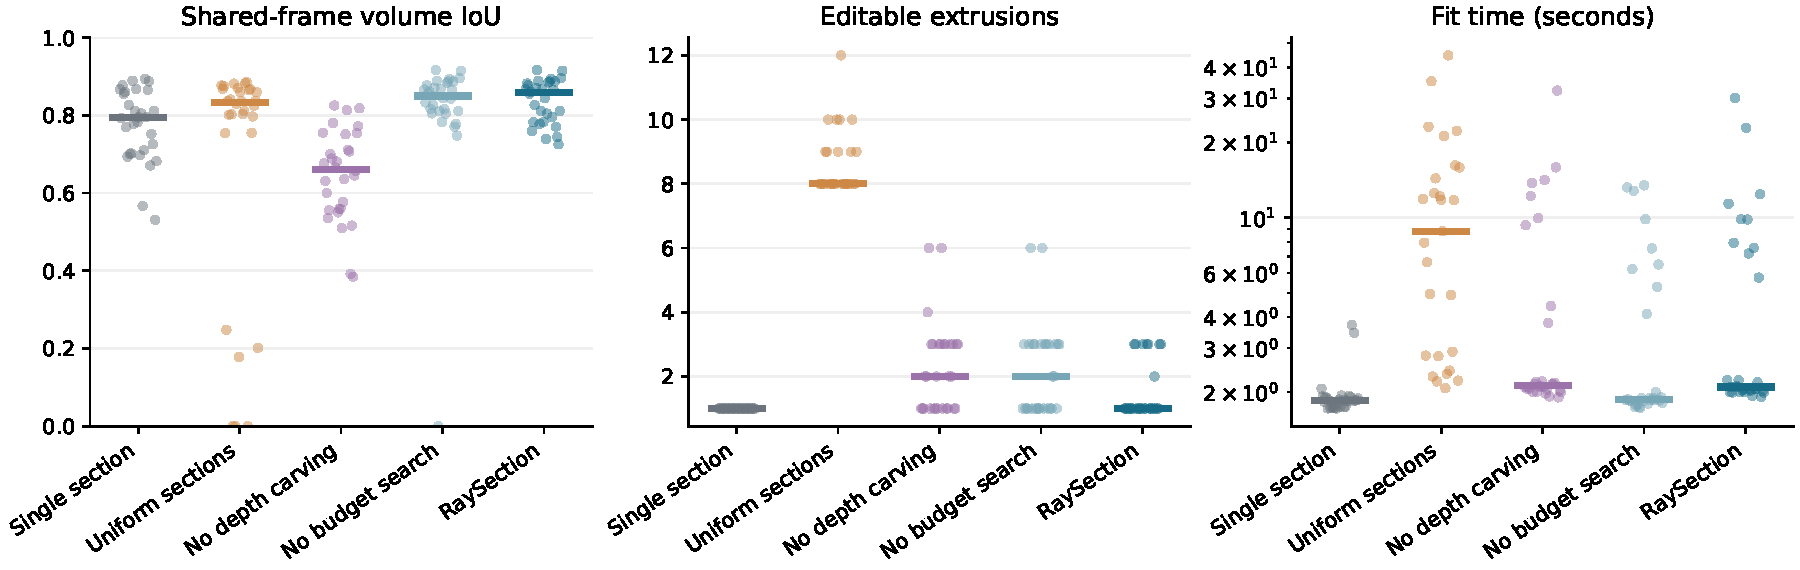
\includegraphics[width=\linewidth]{../../docs/assets/ray_sections/quantitative.pdf}
\caption{Per-instance controlled outcomes. Points are individual procedural
instances; horizontal marks show medians. Time includes isolated CAD compilation
and failed candidate attempts, not data generation. Log time scale.}
\end{figure}

\begin{figure}[p]
\centering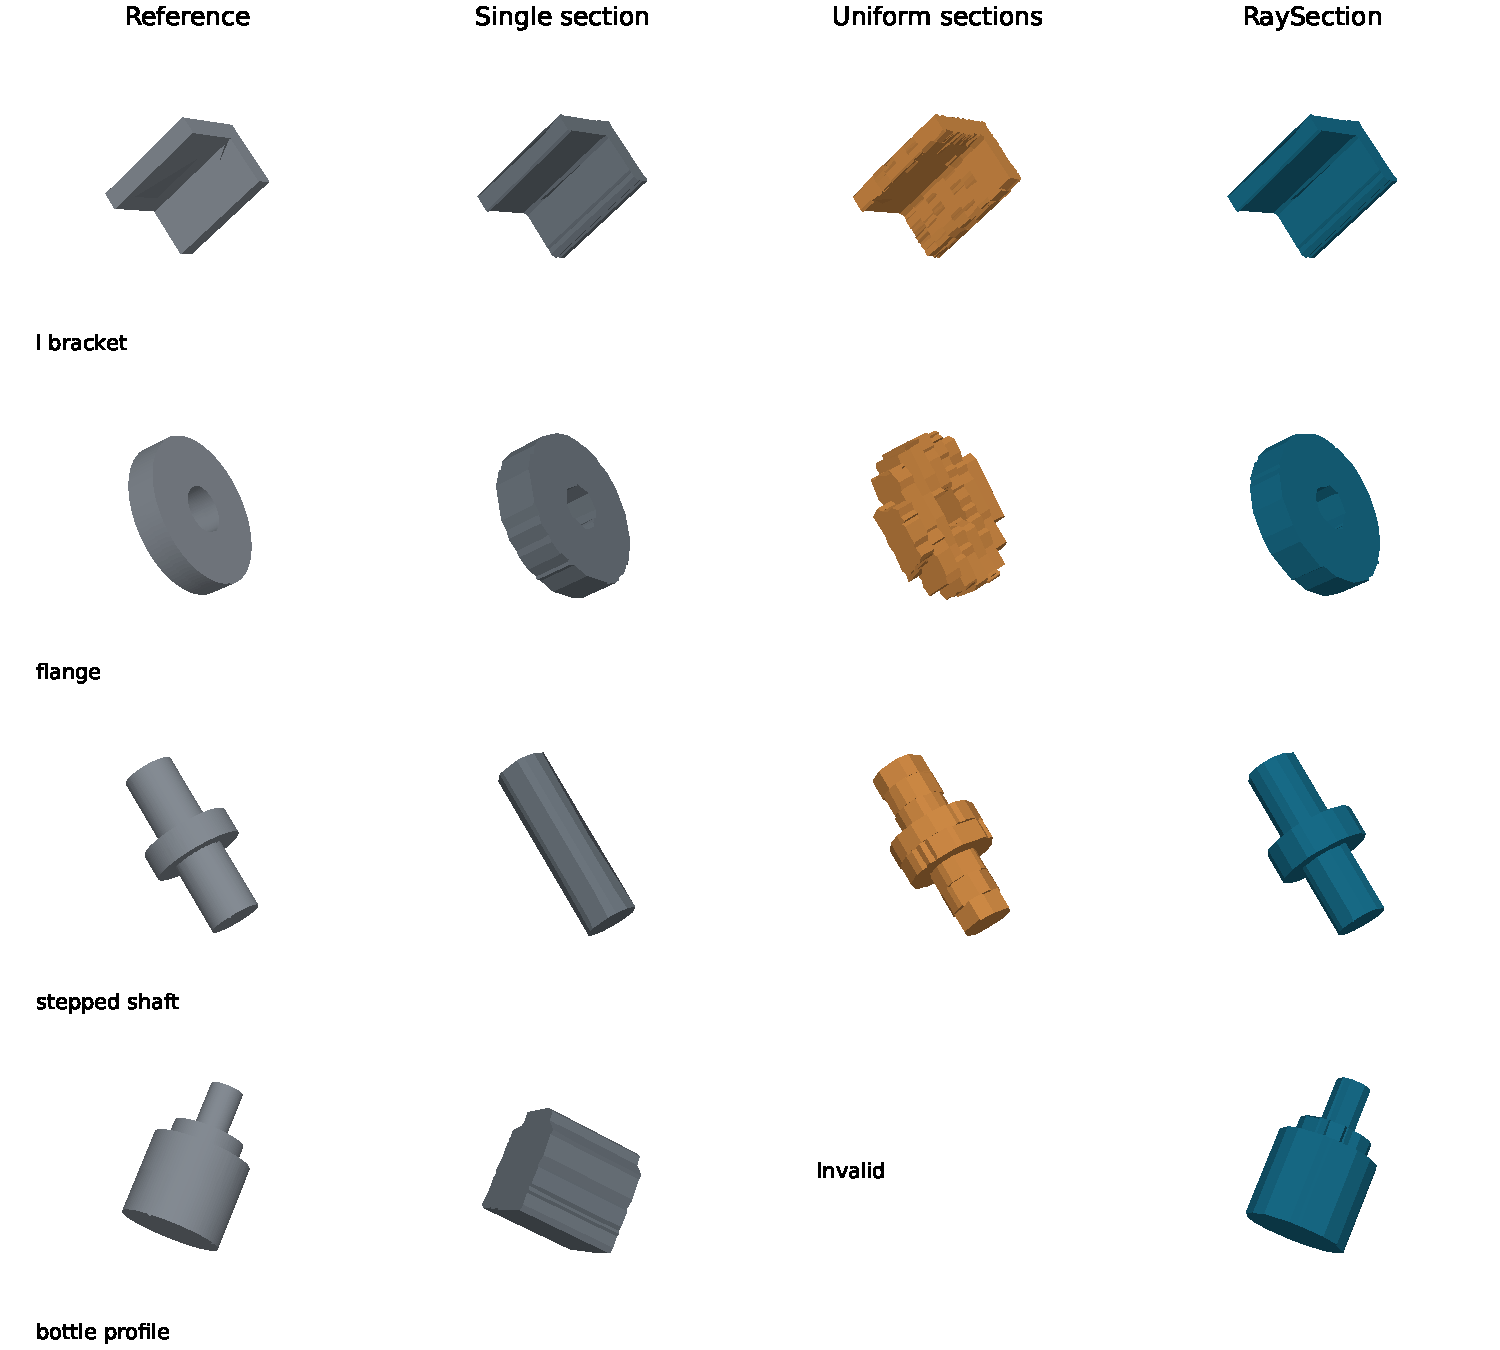
\includegraphics[width=.98\linewidth]{../../docs/assets/ray_sections/qualitative.pdf}
\caption{Shared-frame qualitative comparison on the first generated L-bracket,
flange, stepped-shaft and bottle-profile instances. Rows were selected by family
and generation index, not by measured improvement. Polygonal profiles and
stair-step approximations remain visible limitations.}
\end{figure}

\begin{table}[t]
\centering\small\begin{tabular}{lrrrrl}
\toprule
Case & v9 view IoU & Ours view IoU & Ours depth & Ours edge P & Decision \\
\midrule
o02-fixed & 0.891 & 0.875 & 0.971 & 0.284 & ABSTAIN \\
o04-fixed & 0.862 & 0.896 & 0.987 & 0.291 & ABSTAIN \\
o10 & 0.680 & 0.334 & 0.370 & 0.447 & ABSTAIN \\
o20-fixed & 0.755 & 0.413 & 0.472 & 0.416 & ABSTAIN \\
o25 & 0.880 & 0.839 & 0.904 & 0.354 & ABSTAIN \\
\bottomrule
\end{tabular}

\caption{Exploratory real RGB. View IoU and depth use the eight views excluded
from the new fitter; edge precision and final decisions use the full verifier.
The historical system used all views during fitting. These values measure
source agreement, not reference-CAD accuracy or hidden-topology correctness.}
\label{tab:real}
\end{table}

Executable budget search produced 5/5 kernel-valid candidates, compared with 2/5 for the best-partition-only variant. Only 0/5 candidates passed every existing source-view gate. Table~\ref{tab:real} therefore supports an integration and executability result, not reliable real-photo CAD recovery. The historical v9 comparison also remains an exploratory diagnostic. A lower-complexity fallback can regain a valid solid while losing geometric detail; validity is not a monotonic accuracy guarantee.


\section{Limitations and reproducibility}
The representation is a stack of parallel prismatic sections in a selected
frame. Smooth curvature becomes polygonal or stepped; oblique interacting
features can require many sections. The procedure produces editable coordinates
and heights, not semantic constraints, circles, fillets, tolerances or a recovered
designer feature tree. Its finite frame proposals and largest-component filter
can discard real structure. Ray thresholds assume reasonably calibrated masks
and depth; transparency, specularity, motion and inconsistent MVS can invalidate
those assumptions. Hidden cavities remain unidentifiable without observations.

The controlled data favor prismatic and stepped families. Exact synthetic masks
and calibration simplify the task. Thirty instances from ten generators are too
few to establish broad industrial generalization. The real cases are exploratory
and use oracle target selection. Learned competitors were not rerun. Novelty
claims are limited to the specified implementation and formulation; a focused
literature search cannot establish priority for every component combination.

Code, scripts, source hashes, per-instance ledgers and a generated ray bundle
are released with the DA3-CAD repository. The CLI supports CPU and CUDA and
refuses to overwrite an existing result directory. The measured environment is
Python 3.12, PyTorch 2.13 with CUDA 13 and an RTX 5080 with 16 GB memory.
Some study jobs shared the workstation, so the recorded times are descriptive
end-to-end measurements rather than isolated hardware throughput benchmarks.
The release separates candidate generation from downstream acceptance. No
third-party model weights or T-LESS imagery are redistributed.

\paragraph{AI assistance and review.}
An OpenAI coding assistant contributed algorithm exploration, implementation,
experiment execution, literature lookup, drafting and internal consistency
review under the project maintainer's instructions. Measurements were computed
by the released scripts. Internal critique was same-model self-review, not
independent peer review. The maintainer must confirm authorship and responsibility
before external submission. This report is not a claim of publication acceptance.

\section{Conclusion}
\method{} provides a training-free path from calibrated ray evidence to compact,
executable sketch-extrusion candidates. Exact interval optimization addresses a
restricted approximation problem; budget enumeration and CAD admission address
the separate problem of executable topology. The controlled study quantifies
the resulting accuracy--complexity trade-off, while the real-RGB audit preserves
failures and abstentions. This separation supports reproducible method
development without equating a valid STEP file with a correct reconstruction.

\bibliographystyle{plain}
\bibliography{references}
\end{document}
